Formally evaluating the effectiveness of a meta-toolkit for visual analytics is complex. Arguably the most convincing method would require two groups of programmers of equivalent skills to implement the same set of visual analytics programs with and without Obvious. Then, a judgment could be made from the time spent and the quality of the results. This methodology has been used to assess the InfoVis Toolkit [4] with students but is impractical for real Visual Analytics applications that are more complex and would not fit the scope of student projects.

Another method, used to validate Prefuse [3] would be to re-implement complex Visual Analytics applications using Obvious and assess the results, again in term of time and quality. This is what we have done and we report on our results here.

\subsection{Coding applications with Obvious}

This section will show how Obvious can implement well know examples of information visualizations techniques introduced in several toolkits such as prefuse and Infovis toolkit by combining different Obvious components.

The two first examples use two different implementations (obvious-ivtk and obvious prefuse) to illustrate the same use case : display of a Network using the standard graph layout of the targeted implementation. The third example demonstrates how to create an application by combining component from different Obvious implementations.

The first step is to create an Obvious data structure. We have chosen to illustrate two ways of creating an Obvious structure : one is to wrap an existing data structure into an Obvious one, another is to read a file using a common format (CSV, GraphML...). As shown, in the code sample, factories are provided for each implementation and they allow the developer to use the convenient strategy to set up the data structure. 

Once the data is ready, the next step is to create the visualization. As explained in the Visualization section,  to create the Obvious Visualization, it is needed to provide additional parameters such as the label column used to display nodes in the first two examples. For the scatterplot example, columns used for X and Y axis are indicated in the map of parameters.

Finally,  created Visualizations are injected in a View component. Since all examples use Swing, they are added to Jframes and then those frames are displayed to the final user. It is also possible to add zoom and pan control to created views in order to add interactivity to those examples.

\lstset{basicstyle=\small,language=Java,caption={Visualizing a graph with Obvious},label=codeSample1}
\begin{lstlisting}
/*
* Creates the graph structure.
*/
infovis.Graph g = Algorithms.getGridGraph(10, 10);
Network network = new IvtkObviousNetwork(g);

/*
* Creates the associated visualization using the factory
* for visualization.
* I specify no predicate and no extra parameter.
*/
Visualization vis = new IvtkVisualizationFactory()
    .createVisualization(network, null, "network", null);

/*
* Creates the view.
*/
view = new IvtkObviousView(vis, null, null, null);
JFrame frame = new JFrame();
JScrollPane panel = new JScrollPane(view.getViewJComponent());
frame.add(panel);
frame.pack();
frame.setDefaultCloseOperation(JFrame.EXIT_ON_CLOSE);
frame.setVisible(true);
\end{lstlisting}

\lstset{basicstyle=\small,language=Java,caption={Combining different Obvious implementations to display a scatterplot},label=codeSample2}
\begin{lstlisting}
// Defining the data factory to use,
// obvious-prefuse will be used for the data structures.
System.setProperty("obvious.DataFactory",
    "obvious.prefuse.PrefuseDataFactory");
// Creating an Obvious CSV reader and loading an Obvious table
CSVImport csv = new CSVImport(new File(
    "src//main//resources//articlecombinedexample.csv"), ',');
Table table = csv.loadTable();
// Creating the parameter map for the monolithic object.
Map<String, Object> param = new HashMap<String, Object>();
param.put(PrefuseScatterPlotViz.X_AXIS, "id"); // xfield
param.put(PrefuseScatterPlotViz.Y_AXIS, "age"); // yfield

// Creating the visualization then the view...
Visualization vis = new IvtkScatterPlotVis(table, null,
    null, param);

IvtkObviousView view = new IvtkObviousView(vis,  null, "scatterplot", null);
JFrame frame = new JFrame("");
frame.setDefaultCloseOperation(JFrame.EXIT_ON_CLOSE);
frame.add(view.getViewJComponent());
frame.pack();
frame.setVisible(true);
\end{lstlisting}
\subsection{Example using Weka}

Weka is a software suite of machine learning. It has been proven useful to design such applications, even in visual analytics. That is why in the obviousx package (utils), we have chosen to introduce mechanisms to support Weka. So, in practice, with one line of code, it is possible to create a Weka Instances (Weka data structure) from an Obvious table. Thus, each toolkit implementing Obvious can be easily linked with Weka.

\subsection{EdiDuplicate (a DDupe-Like application)}

INRIA maintains a database for the publication of its member. Researchers regularly fill this database, called HALINRIA, with their new publications. However, mistakes often appears during this process: duplicated authors, institutions or papers. That is why Obvious has been used
to create a DDupe like application to detect duplicated authors in the database.

DDupe is a software initially written in .NET dedicated to detect and merge duplicated nodes (often modeling people)  in (social) network to facilitate data analysis. It uses similarity metric to compare each pair  of authors and class results in descending order of similarity. In addition, DDupe allows the user to see the neighbourhood of the pair of nodes before merging them, in order to check if common nodes exist among their neighbors and then to confirm metric results.

\begin{figure}
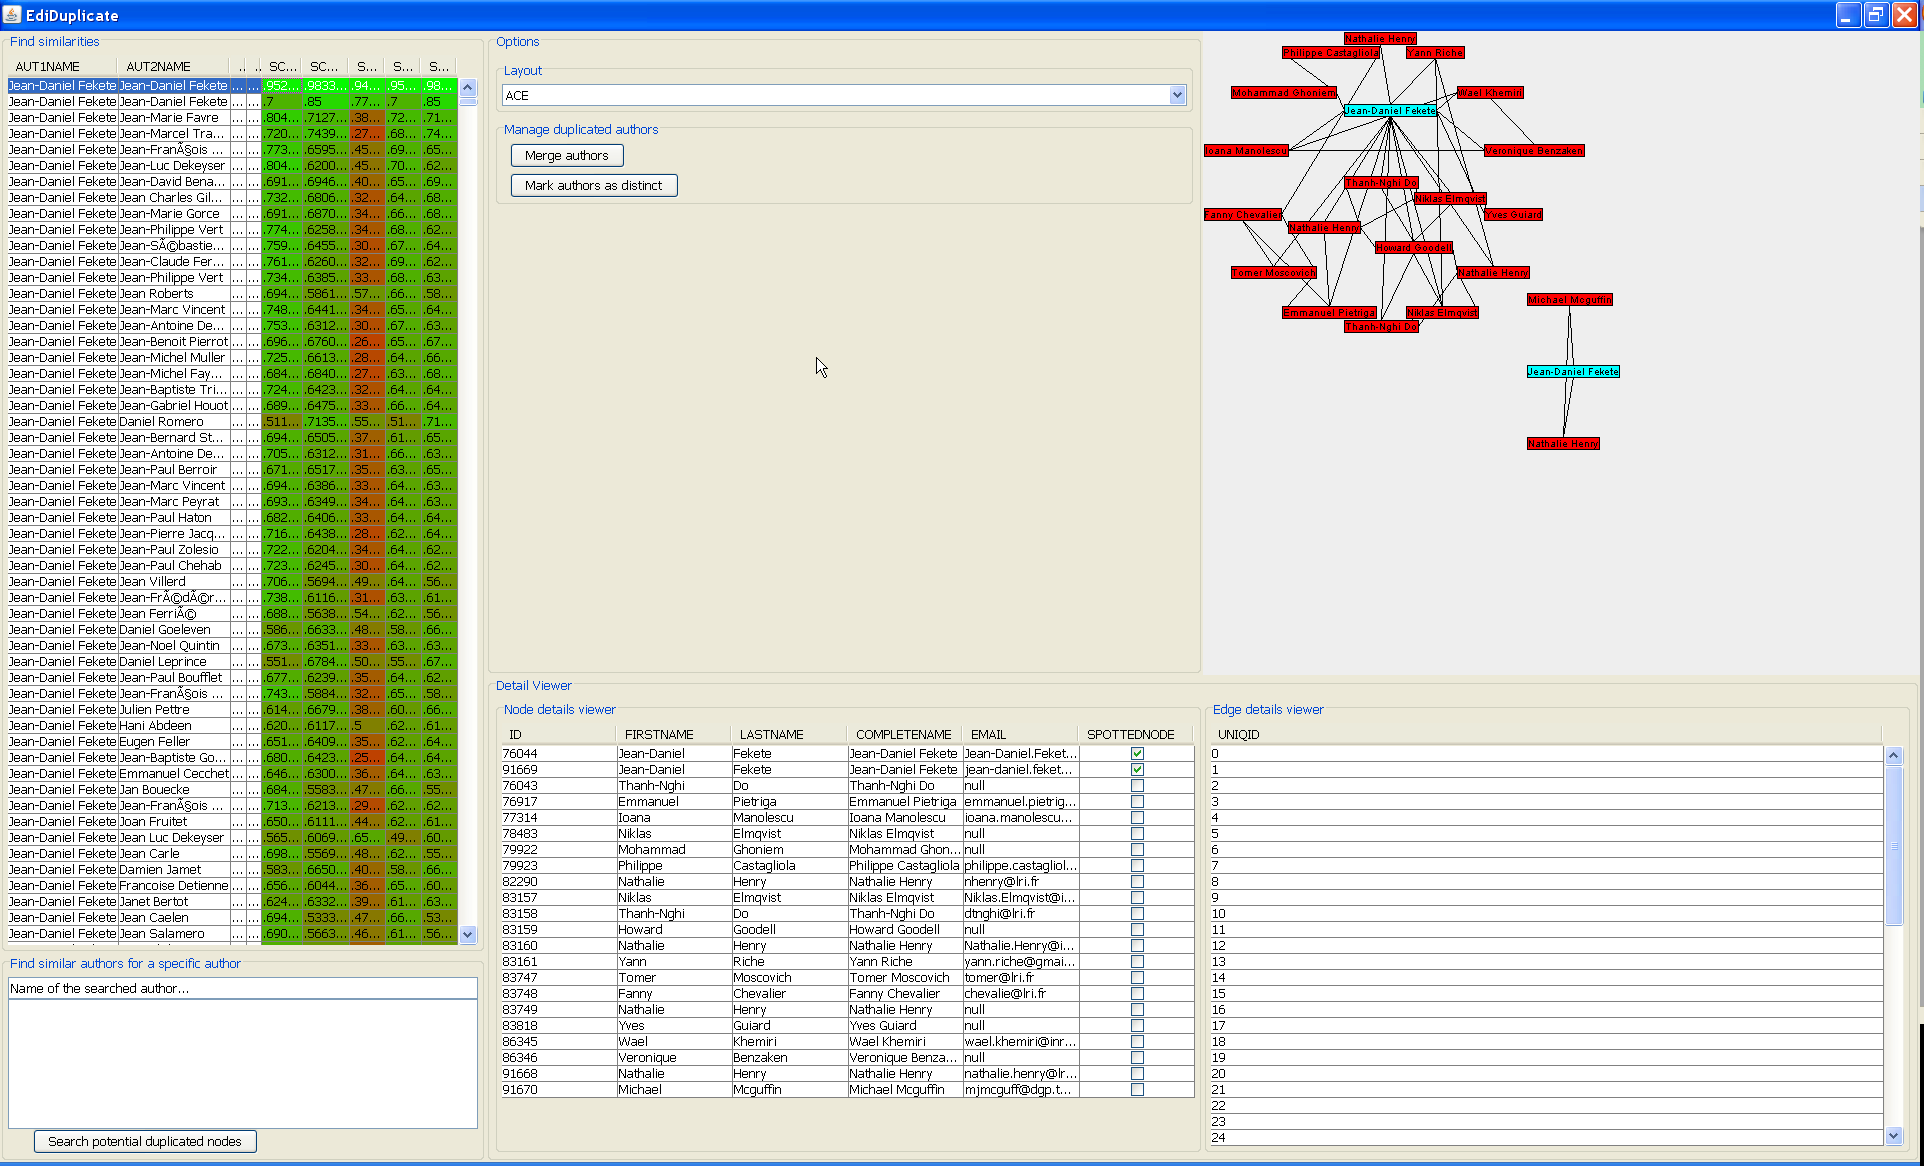
\includegraphics[width=\columnwidth]{figures/ediduplicate}
\caption{A screenshot of Ediduplicate}
\label{fig:ediduplicate}
\end{figure}

Our application EdiDuplicate offers the same possibilities but with extensions to cover specific needs. Concretely, we have implemented a loader to create an Obvious network from the  database. This structure is then fed by an external application with metrics for each pair of authors. Then, those statistics are displayed in a JTable (automically created from the Obvious structure). When, the user clicks on a cell a view of the neighbourhood of the current nodes is created. Then, with this information, the user is able to decide if the potential duplicated authors has to be merged. In addition, it is possible to query the Obvious structure to only display pair of duplicates for a specific authors. The user can also change the layout used to display the neighbourhood network with a JList: all graph layouts introduced in Infovis Toolkit are available. 

Concretely, the application mainly combines Obvious components and Swing components (derived from Obvious structure). For the data model, an Obvious Network is used (from the obvious-ivtk implementation), the visualization and the view part are also provided by this implementation. Building this application takes about less than a week.
